\chapter{Tests Results}
\label{ch:tresults}

\section{Package functionality testing}
Testing an integration/translation Package, and this one specifically, is a rather complex task to evaluate as Bird configuration files are modular and desired settings can be achieved in different ways.
Even more, although an \textit{it works/it does not work} policy could be accepted, it does not mean that there are no other possible implementations that could work in a better way.
For example, filters and functions can be either written in the \textit{.conf} file or included using \texttt{\%include} mechanism, being the second one a better approach as it enhances code readability as well as it avoids bloating the configuration file unnecessarily.

With this introduction in mind, the following sections will explain how this package has been tested following Bird's configuration base requirements and service behaviour and some \textit{future work} ideas to achieve automatic and unit tests.


\subsection{Configuration of the \textit{translation} tests (future work)}
To perform configuration integrity tests in current package, it is required to repeat the execution of \texttt{/etc/bird\{4|6\}/init.d/bird4 restart} in order to trigger the UCI-bird.conf translation from a target UCI file. The code to do this translation has been refactored in an functional manner to allow future unit tests or, at least, make it easier to integrate it in an automated test framework or process. For example, an automated CI/CD build process could build an update of the package, push it into a test node, execute the translation process and compare it against the previous (or a stable) version, as well as check its correctness by querying Bird's status.

\subsubsection{Reviewing v0.2 against v0.3}
Testing the outputs from the old and new packages, and taking into account that there are some manual changes in the old one, the following example is configured as follows:

\begin{itemize}
    \item Router IDs follow node's IP Address.
    \item Kernel, Device and Static Protocols have been set by default.
    \item A Static Route has been added  (identical).
    \item BGP Template and Instance have been configured following v0.2 scheme with matching settings to avoid Bird failures.
    \item BGP Instance AS and Neighbours are dummy values.
    \item A BGP Filter called "all\_ok" (accept all routes) has been added using each version's process.
\end{itemize}

In the new package, we have instantaneous configuration correctness feedback as we can check Bird's status in the Status Page. 
In the old package, after executing \texttt{/etc/bird\{4|6\}/init.d/bird4 start}, Bird will fail and it is required to move the Filter "all\_ok" to the top of the document. Bird will start correctly after this modification.

After checking that both daemons are running, we can then perform a \textit{diff} between the configuration files and look for any noticeable difference.

\begin{lstlisting}[language=diff,caption={Differences in Bird configuration using v0.2 and v0.3 of the Package.}]
3,9d2
<    #Filter filter1:
<    filter all_ok
<    {
<        accept "all ok";
<    }
<
13c6
<    router id 192.168.1.200;
---
>    router id 192.168.1.100;
17a11,17
>    #Functions Section:
>    #End of Functions --
>  
>    #Filters Section:
>    include "/etc/bird4/filters/filter1";
>    #End of Filters --
>  
19c19
<    protocol kernel {
---
>    protocol kernel kernel1 {
46c45
<    source address 192.168.1.200;
---
>    source address 192.168.1.100;
57c57
<    neighbor 192.168.1.201 as 1002;
---
>    neighbor 192.168.1.101 as 1002;
\end{lstlisting}

As shown in this \textit{diff} snippet, almost all the translated configuration is identical apart from:

\begin{itemize}
\item Different Router IDs and BGP neighbours (expected)
\item Kernel Protocol definition (minor change in the API)
\item BGP Filter definition (major change in the API)
\end{itemize}

\subsection{Bird Daemon Errors}
Bird Daemon provides an error exit code together with different text outputs in order to highlight errors in the configuration. Although most of the times it can be easily spotted using Bird's feedback, there are also instances where the Daemon's documentation may be required to fix them.

\subsubsection{Bird Daemon Error examples}
The most common errors that an administrator may need to resolve are:

\begin{itemize}
\item A configured field has incorrect syntax.
Bird will give you hints about what is wrong most of the times: wrong IP address format \texttt{bird: /tmp/bird4.conf, line 7: Invalid IPv4 address 1921.68.1.1}. But some \textit{rare} times the message is less helpful and you may need to check the contents of the file and understand the error.

As an example of this: \texttt{bird4: Failed - bird: /tmp/bird4.conf, line 65: syntax error}. We need to check the bird4.conf file and see that in line 65:

\begin{lstlisting}[language=bash, caption={Bird4.conf contents}]
64:    protocol bgp BGPExample {
65:        import Filter NonExistingFilter;
66:    }
\end{lstlisting}

We will need to find out that the shown filter used in the import field of BGP Protocol, does not exist.

\item Non-compatible configuration.
The other set of common errors is non-compatible fields in a Protocol.

As an example of this: \texttt{bird: /tmp/bird4.conf, line 76: Only internal neighbor can be RR client}. We need to remove the Route Reflector Client setting from the BGP Instance to fix this behaviour.

\item Missing filter or function.
If you include a filter name in any of the Protocols or if any of your filters use a non-existing function, Bird will fail to start showing an error as follows: \texttt{bird: /tmp/bird4.conf, line 71: No such filter}.

\item Syntax errors in a filter or function.
This error follows the same approach as the first bullet: \texttt{bird: /etc/bird4/filters/filter-20170507-0951, line 4: syntax error}. You are required to go to command line and fix the problem checking the configuration and filter or function files.

\item Filter calling to non-existing functions.
If your filter executes a command that is not defined by Bird's syntax, it will handle it as a function. If that function does not exist in any of the handled files, it will show this error: \texttt{bird: /tmp/bird4.conf, You can't call something which is not a function. Really.}

\item Filters not accepting/rejecting routes.
Bird Daemon filters must return an \textit{accept} or \textit{reject} policy per route received. If any of your filters does not return any policy per route, it will be silently ignored and substituted with an "accept".

As an example of this issue:
\begin{lstlisting}[language=bash, caption={Filter printing message}]
filter doNothing
{
    print "HelloWorld";
}
\end{lstlisting}

Bird Daemon will succeed starting up but, if we check the log information in the Log Page, this error message will be shown:
\begin{lstlisting}[language=bash, caption={Filter printing message.}]
<ERR> Filter doNothing did not return accept nor reject. Make up your mind
<INFO> HelloWorld
\end{lstlisting}

\end{itemize}


\section{Package's behaviour testing} 
\subsection{Simple Scenario: Single BGP Session connected to Guifi.net}
As part of the acceptance tests, a VM was set up by a sysadmin in UOC's network to act as a pre-production machine. This VM is connected to a \textit{Mikrotik} Router acting as Gateway to \textit{Guifi.net} but this scenario does not connect or communicate through any Mesh Network using BMX6, so it is an end point. More detailed information an a graphic is available on section \ref{sub:sub:idt}.

The configuration of this system is almost identical, component-wise, to the ones available in Guifi.net. However, this system will only export its own route and import any received.

Bird UCI configuration set through the web UI and its translation into Bird4 configuration can be reviewed in appendix \ref{app:ch:bdcuoc}. After setting up the BGP session, we have started receiving 3000+ routes and exporting our own:

\begin{lstlisting}[language=bash,caption={Bird BGP query.}]
root@LEDE-eloi:~# birdcl4 show protocols all
[...]
BGPImportALL BGP      master   up     2017-05-10  Established
  Preference:     100
  Input filter:   ebgp_in
  Output filter:  ebgp_out
  Import limit:   3000 [HIT]
    Action:       warn
  Routes:         2999 imported, 1 exported, 2999 preferred
  Route change stats:     received   rejected   filtered    ignored   accepted
    Import updates:        1208383          0          0         88    1208295
    Import withdraws:       337268          0        ---        300     336968
    Export updates:        1208298    1208295          2        ---          1
    Export withdraws:       336968        ---        ---        ---          0
  BGP state:          Established
    Neighbor address: 172.25.35.25
    Neighbor AS:      59361
    Neighbor ID:      10.90.224.65
    Neighbor caps:    refresh AS4
    Session:          external AS4
    Source address:   172.25.35.26
    Route limit:      2999/3000
    Hold timer:       160/180
    Keepalive timer:  29/60
\end{lstlisting}

Using Bird Remote Control we can verify Bird's BGP instance. As key information:

\begin{itemize}
    \item BGP Instance: BGPImportALL
    \item Filters applied: \textit{ebgp\_in} and \textit{bgp\_out} to allow only Guifi.net routes (\texttt{10.0.0.0/8}).
    \item We are connected to our neighbour 10.90.224.65 with Autonomous System ID 59361
    \item  The number of routes received fluctuates but the data shown presents exactly 2999 routes imported, but this number fluctuates.
    \item This fluctuation has already reached our configured Import Limit (HIT) and that generated warnings.
    From our Package's Log Page:
    \texttt{2017-05-21 22:09:13 <WARN> Protocol BGPImportALL hits route import limit (3000), action: warn}. It has been configured to warn the administrator, but Bird allows it to be set to block the protocol.
    \item As an endpoint with no extra routes, we are exporting just one.
\end{itemize}

As a health check, we can query Bird of its last reconfiguration, reboot time or status using \texttt{bircl4 status}:

\begin{lstlisting}[language=bash,caption={Bird status query.}]
root@LEDE-eloi:~# birdcl4 show status
BIRD 1.6.3 ready.
BIRD 1.6.3
Router ID is 10.139.173.161
Current server time is 2017-05-22 00:20:23
Last reboot on 2017-05-10 19:31:09
Last reconfiguration on 2017-05-10 19:31:09
Daemon is up and running
\end{lstlisting}

Some examples of this BGP session working are the following:

\begin{itemize}
    \item \texttt{Traceroute} to the node BCNLlenguadoc17Rack. Node close to our node:
\begin{lstlisting}[language=bash, caption={Traceroute from LEDE-MXN1 to BCNLlenguadoc17Rack.}]
root@LEDE-MXN1:~# traceroute 10.1.56.193
traceroute to 10.1.56.193 (10.1.56.193), 30 hops max, 46 byte packets
 1  10.90.224.65 (10.90.224.65)  0.335 ms  0.258 ms  0.204 ms
 2  10.139.92.129 (10.139.92.129)  1.004 ms  0.911 ms  0.882 ms
 3  10.38.140.225 (10.38.140.225)  2.467 ms  2.508 ms  6.913 ms
 4  10.139.95.97 (10.139.95.97)  4.369 ms  4.054 ms  3.815 ms
 5  10.1.56.193 (10.1.56.193)  8.352 ms  6.813 ms  8.098 ms
\end{lstlisting}
    \item \texttt{Traceroute} to the node AV-Ajuntament-Avinyonet. This node is located in the Hall of a village located about 50km from Barcelona.
\begin{lstlisting}[language=bash, caption={Traceroute from LEDE-MXN1 to AV-Ajuntament-Avinyonet.}]
root@LEDE-MXN1:~# traceroute 10.139.62.163
traceroute to 10.139.62.163 (10.139.62.163), 30 hops max, 46 byte packets
 1  10.90.224.65 (10.90.224.65)  0.250 ms  0.372 ms  0.327 ms
 2  10.139.92.129 (10.139.92.129)  0.906 ms  0.800 ms  1.438 ms
 3  10.38.140.225 (10.38.140.225)  2.560 ms  2.819 ms  2.063 ms
 4  10.38.141.65 (10.38.141.65)  2.638 ms  2.956 ms  2.421 ms
 5  *  *  *
 6  10.90.150.81 (10.90.150.81)  4.022 ms  7.174 ms  4.112 ms
 7  10.139.62.163 (10.139.62.163)  10.031 ms  11.963 ms  8.288 ms
 8  10.139.62.163 (10.139.62.163)  9.779 ms  9.629 ms  7.286 ms
\end{lstlisting}
    \item \texttt{Traceroute} from the external node BCNLaFabraRd1:
\begin{lstlisting}[language=bash, caption={Traceroute from BCNLaFrabraRd1 to LEDE-MXN1.}]
root@BCNLaFabraRd1:~# traceroute 10.90.236.97
traceroute to 10.90.236.97 (10.90.236.97), 30 hops max, 38 byte packets
 1  10.1.56.193 (10.1.56.193)  9.776 ms  5.078 ms  2.970 ms
 2  10.139.95.97 (10.139.95.97)  10.313 ms  10.732 ms  6.101 ms
 3  10.38.140.225 (10.38.140.225)  12.552 ms  10.050 ms  7.185 ms
 4  10.139.92.129 (10.139.92.129)  15.783 ms  7.721 ms  9.526 ms
 5  10.90.224.65 (10.90.224.65)  29.962 ms  13.571 ms  16.453 ms
 6  10.139.173.161 (10.139.173.161)  11.361 ms  9.258 ms  9.721 ms
\end{lstlisting}
\end{itemize}

\newpage
\subsection{Target Network Scenario: Final package complete testing}
\label{sub:fulltest}
As introduced in the section \ref{sub:sub:fpt}, a number of virtual nodes and network resources have been created in order to be able to test the final package in a network almost identical to our target one. This network's configuration has been really challenging because it reflects the complexity that we could find in any other real network, including issues as: to require tunnels to pass through external networks, use of virtual resources to generate specific topologies, external firewalls rules blocking our target network's traffic, etc. Although it has required a lot of debugging in order to align the network's configuration and leave it in the right state to test our Package, all this modifications are out of the scope of the project and are recorded here for reference and better understanding of what a network administrator is required to do.

All the configuration files modified to do this test are available in the Appendix \ref{app:ch:full} separated by node.

The following items will describe the main challenges faced during this environment's creation and alignment:
\begin{itemize}
    \item External Firewall's changes have been required to allow the correct communication between the nodes MXN1 and MXN2  to their respective Guifi.net Peers.
    \item BMX6 protocol has been configured in each node of the mesh network.
        \begin{itemize}
            \item All: export node's internal network (\texttt{10.90.236.X/27}) and import any Guifi.net route (\texttt{10.0.0.0/8}).
            \item Mesh Exchange Nodes: advertise the Guifi.net network (\texttt{10.0.0.0/8}) to the internal nodes, representing themselves as \textit{gateways} to the extenal network.
            \item BMX6's Table Plugin has been set to use the Kernel Routing Table \texttt{251}. By forcing BMX6 to use a specific Kernel Routing Table, Bird is capable to use that specific Kernel Routing Table and exchange routes with BMX6.
            \item Specific Firewall rules have been set in order to permit BMX6 traffic (add \texttt{option device 'bmx+'} to the \texttt{WAN Zone}), thus allowing transit.
        \end{itemize}
     \item An L2TP Tunnel has been configured between the second Mesh Exchange Node (MXN2) and UPF's Guifi.net node. This has been required to pass through UPF's private network and connect to Guifi.net.
\end{itemize}

Once all these external elements are configured correctly, we can start defining and configuring all the required configuration that applies to this project's scope.
\begin{itemize}
    \item Kernel Routing Tables and interfaces.
    \item BGP Peers
    \item Bird Internal pipes to communicate Bird Routing Tables
\end{itemize}
For this section, we will assume that the network settings are configured as shown in the figure \ref{fig:devnet}.


\begin{landscape}
\begin{figure}[ht!]
    \centering
    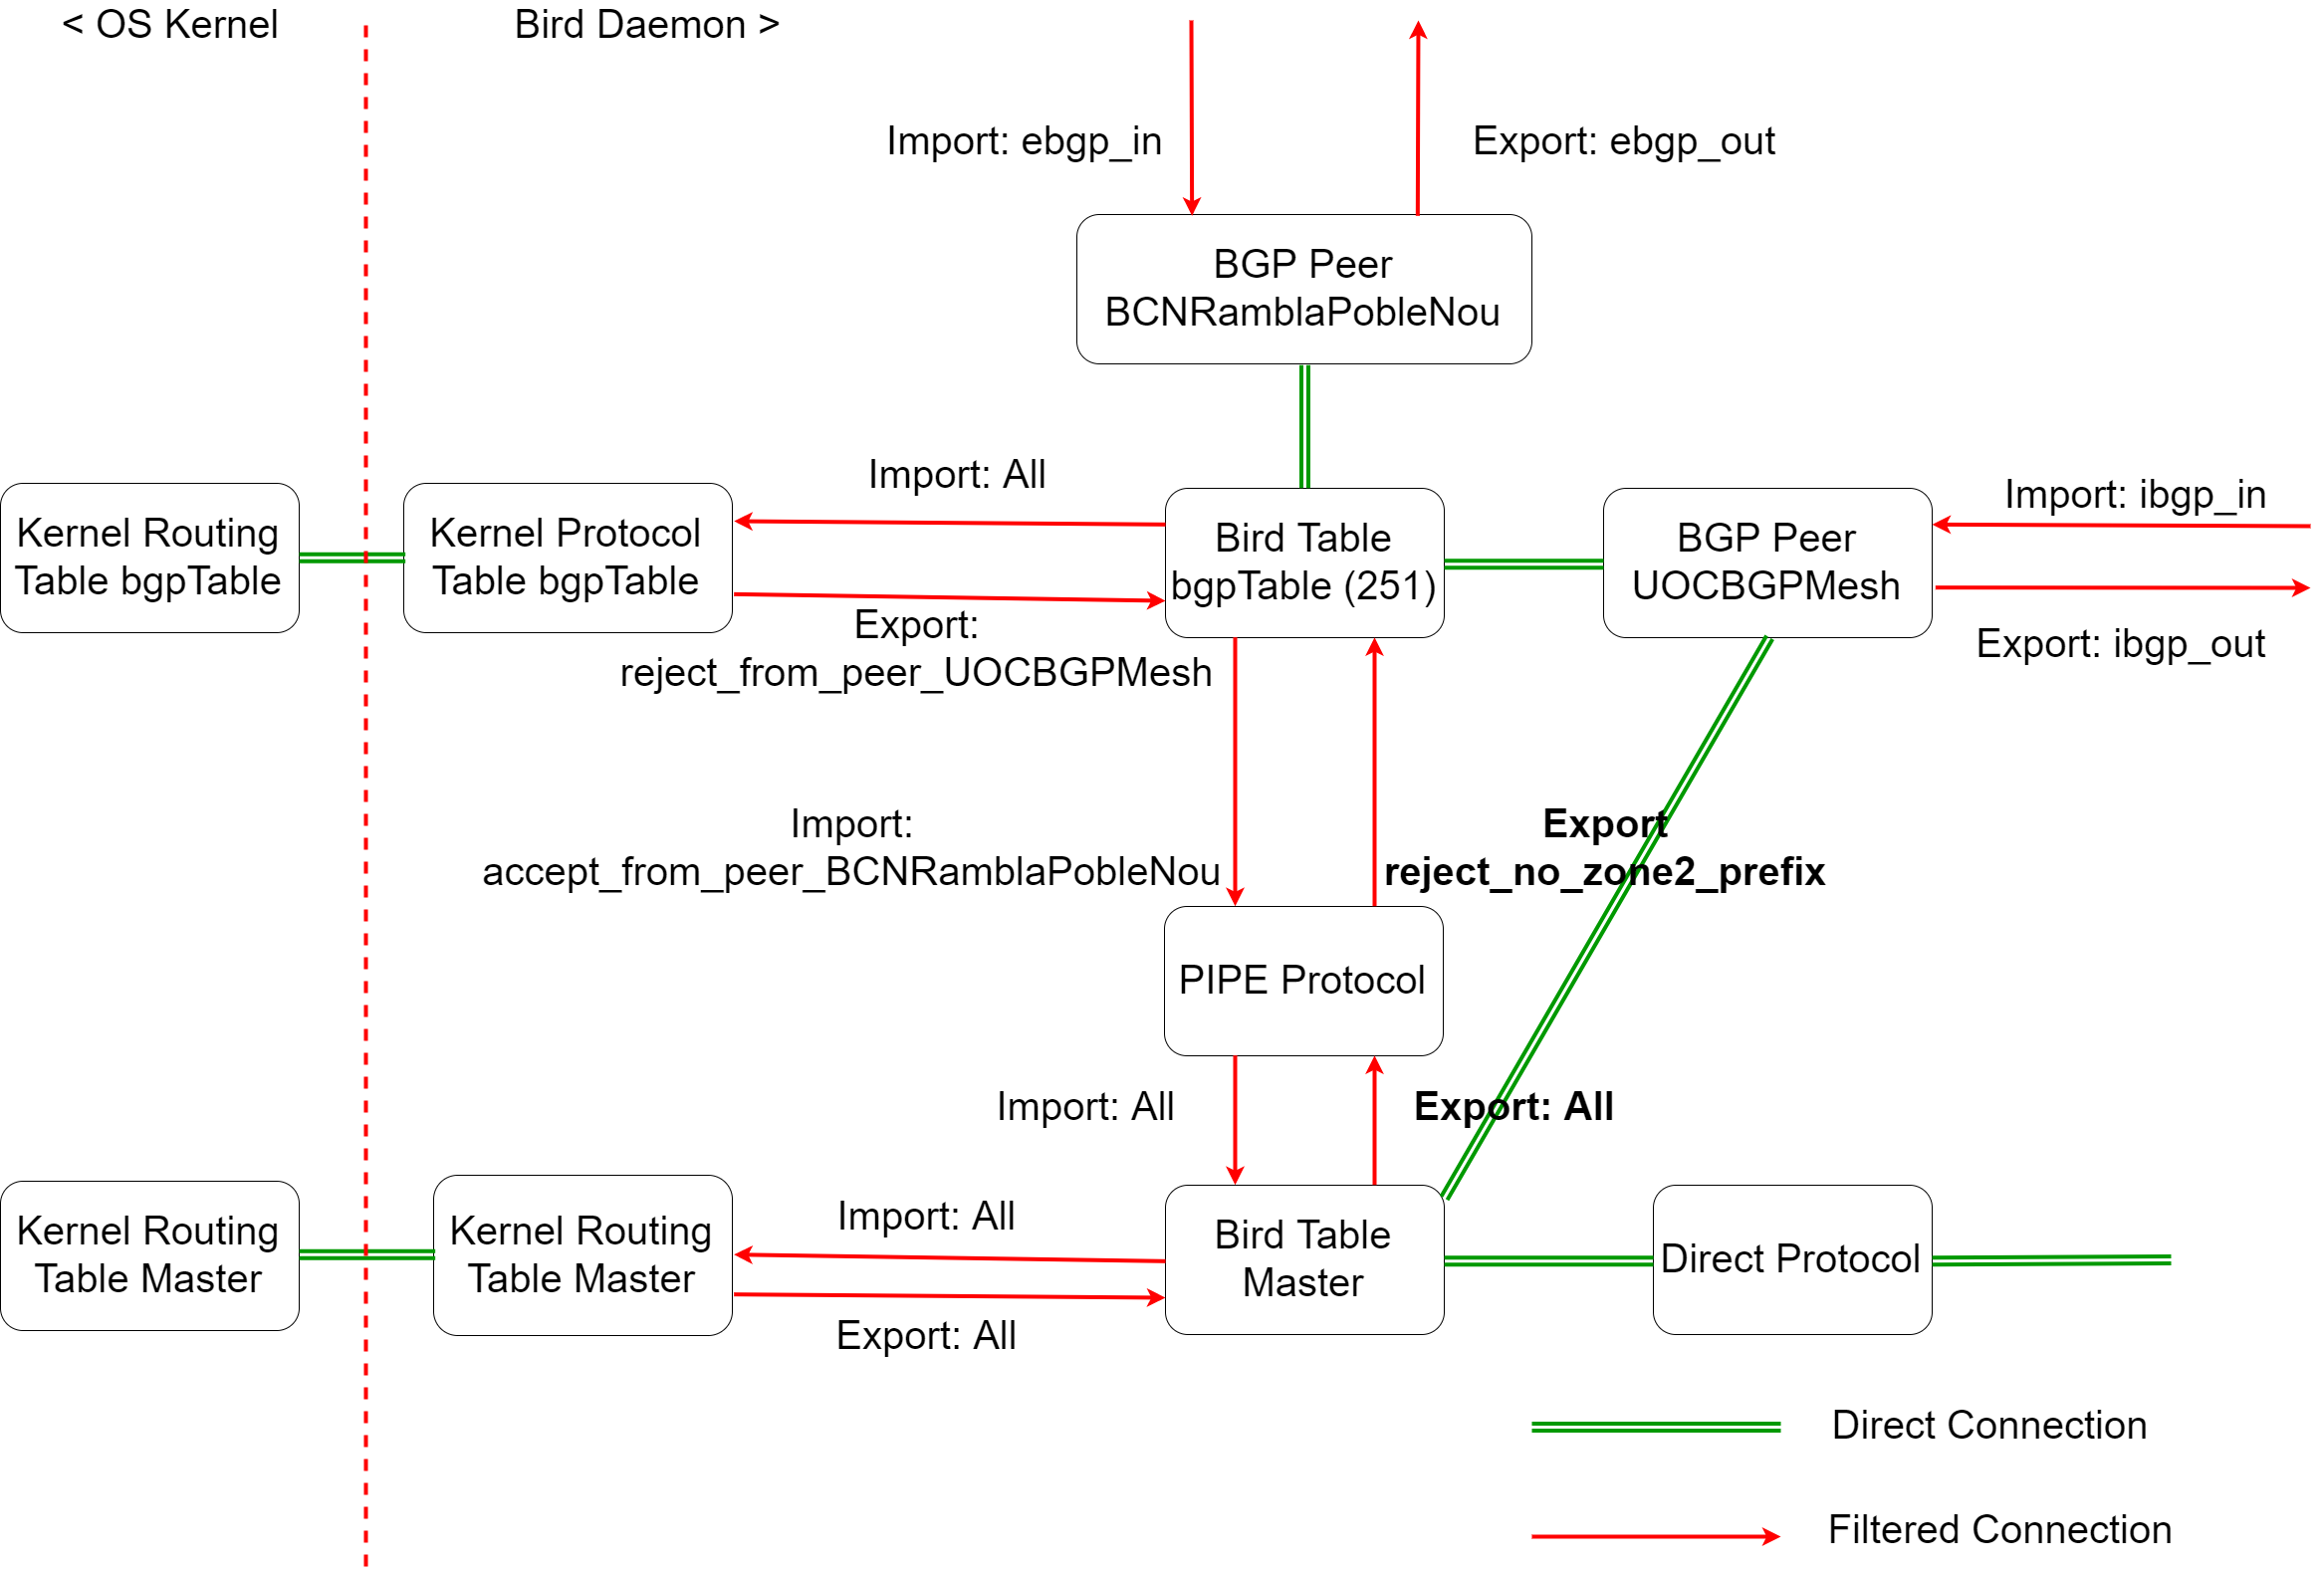
\includegraphics[width=0.7\hsize]{images/tables}
    \caption{Bird Daemon Protocols' configuration.}
    \label{fig:tables}
\end{figure}
This diagram represents MXN1's configuration. However, MXN2's configuration is almost identical apart from being connected to the BGP Peer \texttt{BCNUPFPobleNou}. 
\end{landscape}
\newpage


Summarising this diagram's flow, Bird is configured as follows:

\begin{itemize}
    \item \textbf{Bird Routing Table bgpTable(251)} \footnote{OS Kernel's Routing Table 251 is shared between Bird Daemon and BMX6 Protocol and used to exchange routes.} : this internal table is used by both BGP Peers as their main table. Bird will use this internal table to exchange routes between different internal protocols and tables.
    \item \textbf{Bird Routing Table Master}: this is Bird's default internal table and is used by \texttt{UOCBGPMesh} BGP IGP Session and other Bird protocols.
    \item \textbf{PIPE Protocol}: this internal protocol will exchange routes between the table bgpTable and Master. It is filtered to avoid bgpTable to get any external route available in the Master table.
    \item \textbf{Kernel Protocol for bgpTable}: This protocol will exchange routes between the OS Kernel Routing Table and Bird's bgpTable. It is filtered to avoid the OS Table to get routes from the IGP BGP Session.
    \item \textbf{Kernel Protocol for Master Table}: This protocol will exchange routes between default's OS Kernel Routing Table and Bird's Master Table. This protocol is not filtered because it has already been filtered by the PIPE Protocol.
    \item \textbf{BGP Session UOCBGPMesh}: IGP BGP Session established with the second Mesh Exchange Node. This session will encapsulate the Mesh network as one single AS. This protocol has been filtered in order to allow pass only to Guifi.net prefixes (\texttt{10.0.0.0/8}).
    \item \textbf{BGP Session BCNRamblaPobleNou}: EGP BGP Session established with UOC's Infrastructure Node (our gateway to Guifi.net). This protocol only exports and imports routes from Guifi.net, however, the imported ones will be marked with Router's ID to avoid loops or malfunctioning.
\end{itemize}

After configuring both Mesh Exchange Nodes with the described configuration, the network's behaviour has been tested with successful results shown in the next section. However, a last minute Bug has been found during this test:

\textit{Next Hop Self} is a common BGP attribute used in IGP sessions to fix gateway's advertisements between the AS's internal nodes. This option has been configured on both \texttt{UOCBGPMesh} BGP Sessions, but the routes were not being configured as expected. After reviewing the configuration and comparing it with the translation, it has been found that this attribute was not being propagated. The root cause has been found already (\texttt{get next\_hop\_self} call deleted by mistake) and will be fixed before releasing the code to the community.


\subsubsection{Test Results}
In order to prove the correct behaviour of this configuration, a number of different \texttt{traceroute} actions have been done:

\begin{itemize}
    \item Internal Test: from the Infrastructure Node in UOC's side to the Infrastructure Node in UPF's side:
    \begin{lstlisting}[language=bash, caption={End-to-End  connectivity going through the Mesh Network.}]
[victor@BCNRamblaPoblenou156Rd1] > tool traceroute 10.139.173.65
# ADDRESS                          LOSS SENT    LAST     AVG    BEST   WORST STD-DEV STA..
1 10.90.236.97                       0%    4   0.5ms     0.6     0.5     0.7     0.1      
2 10.90.236.1                        0%    4   0.8ms     0.9     0.7     1.2     0.2      
3 10.139.173.65                      0%    4   2.5ms     2.5     2.4     2.6     0.1
\end{lstlisting}
    As shown in this code snippet, the connection goes from the MXN1 through the mesh to the MXN2 and continues to the UPF Infrastructure Node successfully, thus demonstrating the correct pass of routes through it.
    
    \item External Test (I): Contact external BGP clients from a Mesh client:
    \begin{lstlisting}[language=bash, caption={Mesh node traceroute to node AV-Ajuntament-Avinyonet.}]
root@LEDE-MESH2:~# traceroute 10.139.62.163
traceroute to 10.139.62.163 (10.139.62.163), 30 hops max, 46 byte packets
 1  10.90.236.97 (10.90.236.97)  0.717 ms  0.379 ms  0.788 ms
 2  10.90.224.65 (10.90.224.65)  1.122 ms  0.923 ms  0.494 ms
 3  10.139.92.129 (10.139.92.129)  1.892 ms  1.144 ms  1.022 ms
 4  10.38.140.225 (10.38.140.225)  2.805 ms  2.966 ms  2.824 ms
 5  10.38.141.65 (10.38.141.65)  3.118 ms  3.474 ms  3.255 ms
 6  *  *  *
 7  *  10.90.150.81 (10.90.150.81)  5.244 ms  4.328 ms
 8  10.139.62.163 (10.139.62.163)  50.749 ms  69.197 ms  18.574 ms
 9  10.139.62.163 (10.139.62.163)  56.709 ms  16.521 ms  40.462 ms
\end{lstlisting}
    \item External Test (II): Connectivity test for each Mesh Client:
    \begin{lstlisting}[language=bash, caption={Connectivity test from a Guifi.net Client to each Mesh client.}]
victor@debris:~$ ping 10.90.236.1
PING 10.90.236.1 (10.90.236.1) 56(84) bytes of data.
64 bytes from 10.90.236.1: icmp_seq=1 ttl=58 time=8.35 ms
64 bytes from 10.90.236.1: icmp_seq=1 ttl=58 time=12.57 ms

victor@debris:~$ ping 10.90.236.33
PING 10.90.236.33 (10.90.236.33) 56(84) bytes of data.
64 bytes from 10.90.236.33: icmp_seq=1 ttl=56 time=57.6 ms
64 bytes from 10.90.236.33: icmp_seq=2 ttl=57 time=9.05 ms

victor@debris:~$ ping 10.90.236.65
PING 10.90.236.65 (10.90.236.65) 56(84) bytes of data.
64 bytes from 10.90.236.65: icmp_seq=1 ttl=56 time=70.9 ms
64 bytes from 10.90.236.65: icmp_seq=2 ttl=57 time=7.71 ms

victor@debris:~$ ping 10.90.236.97
PING 10.90.236.97 (10.90.236.97) 56(84) bytes of data.
64 bytes from 10.90.236.97: icmp_seq=1 ttl=57 time=22.5 ms
64 bytes from 10.90.236.97: icmp_seq=2 ttl=57 time=27.9 ms
\end{lstlisting}
\end{itemize}

The next two tests shows an example of what happens if an external client finds a better path (e.g. shorter or with better connection) to go to a specific node which, would avoid our network:

\begin{itemize}
    \item External Peer connected and providing a better path:
    \begin{lstlisting}[language=bash, caption={Route from a Guifi.net client finding a better path to UPF's node.}]
victor@debris:~$ traceroute 10.139.173.65
traceroute to 10.139.173.65 (10.139.173.65), 30 hops max, 60 byte packets
1  192.168.16.1 (192.168.16.1)  0.282 ms  0.511 ms  0.502 ms
2  BCNBenlliure6Rd1--93517.ip.guifi.net (10.228.193.97)  1.491 ms  1.485 ms  1.475 ms
3  BCNSantuari125Rd1--36358.ip.guifi.net (10.228.199.161)  24.481 ms  25.330 ms  25.327 ms
4  BCNRembrandtRB450G--89325.ip.guifi.net (10.139.95.97)  25.318 ms  25.308 ms  25.545 ms
5  HW-AcerRouter--27612.ip.guifi.net (10.38.140.225)  31.905 ms  32.169 ms  32.160 ms
6  BCNUPFp9RB2011--65328.ip.guifi.net (10.139.173.65)  32.150 ms  8.001 ms  7.739 ms
\end{lstlisting}
    As can be seen in route's path, on step 5, the route jumps from AcerRouter to UPF's node, without going through UOC's network.
    
    However, if we disable this node, the client is not able to find better alternative paths and goes through the BMX6 mesh network.
    \item External Peer disconnected and no alternative paths to our network:
    \begin{lstlisting}[language=bash, caption={Route from a Guifi.net client without alternative paths interfering.}]
victor@debris:~$ traceroute 10.139.173.65
traceroute to 10.139.173.65 (10.139.173.65), 30 hops max, 60 byte packets
1  192.168.16.1 (192.168.16.1)  0.282 ms  0.565 ms  0.557 ms
2  BCNBenlliure6Rd1--93517.ip.guifi.net (10.228.193.97)  1.501 ms  1.492 ms  1.482 ms
3  BCNSantuari125Rd1--36358.ip.guifi.net (10.228.199.161)  5.035 ms  5.280 ms  5.270 ms
4  BCNRembrandtRB450G--89325.ip.guifi.net (10.139.95.97)  8.280 ms  8.271 ms  9.841 ms
5  HW-AcerRouter--27612.ip.guifi.net (10.38.140.225)  10.547 ms  10.530 ms  10.526 ms
6  BCNsntJoanMalta51ST1--15065.ip.guifi.net (10.139.92.129)  12.871 ms  8.685 ms  8.375 ms
7  BCNRamblaPoblenou156Rd1--59361.ip.guifi.net (10.90.224.65)  9.045 ms  9.042 ms  13.293 ms
8  BCNRamblaPoblenou156Rd3--92099.ip.guifi.net (10.90.236.97)  11.830 ms  13.261 ms  13.253 ms
9  BCNRamblaPoblenou156Rd6--93730.ip.guifi.net (10.90.236.1)  13.496 ms  16.259 ms  17.499 ms
10  BCNUPFp9RB2011--65328.ip.guifi.net (10.139.173.65)  18.525 ms  17.842 ms  18.505 ms
\end{lstlisting}
    This second time, the client has not found any alternative paths and, after step 5, it jumped to an intermediate node (step 6), to our Infrastructure Node in the UOC (step 7), to our exchange node MXN1 (step 8), to our second exchange node MXN2 (step 9) and finally, it has arrived to the UPF Infrastructure node in step 10.
    
    Comparatively, it is clear and reasonable to avoid 4 extra network hops in comparison to the alternative path.
\end{itemize}
